\documentclass[tikz,border=10pt]{standalone}
\usepackage{tikz}
\usetikzlibrary{positioning, arrows.meta, calc, patterns, decorations.pathreplacing}
\usepackage{amsmath}

\begin{document}
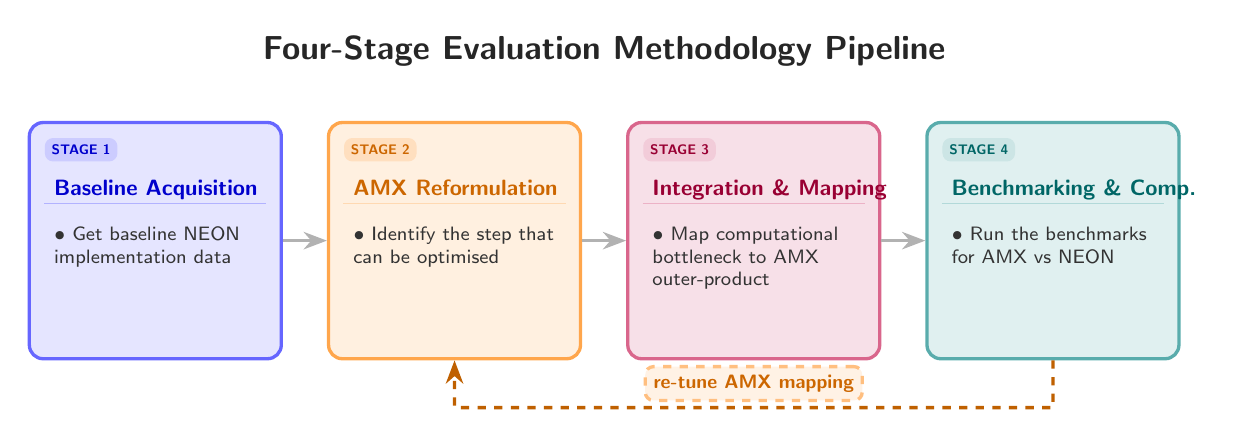
\begin{tikzpicture}[
    >=Stealth,
    font=\sffamily\small,
    box s1/.style={fill=blue!10, draw=blue!60, very thick, rounded corners=5pt,
                   minimum width=32mm, minimum height=30mm, inner sep=6pt},
    box s2/.style={fill=orange!12, draw=orange!70, very thick, rounded corners=5pt,
                   minimum width=32mm, minimum height=30mm, inner sep=6pt},
    box s3/.style={fill=purple!12, draw=purple!60, very thick, rounded corners=5pt,
                   minimum width=32mm, minimum height=30mm, inner sep=6pt},
    box s4/.style={fill=teal!12, draw=teal!65, very thick, rounded corners=5pt,
                   minimum width=32mm, minimum height=30mm, inner sep=6pt},
    badge s1/.style={fill=blue!20, text=blue!80!black, font=\sffamily\tiny\bfseries, rounded corners=3pt, inner sep=2.5pt},
    badge s2/.style={fill=orange!25, text=orange!80!black, font=\sffamily\tiny\bfseries, rounded corners=3pt, inner sep=2.5pt},
    badge s3/.style={fill=purple!20, text=purple!80!black, font=\sffamily\tiny\bfseries, rounded corners=3pt, inner sep=2.5pt},
    badge s4/.style={fill=teal!20, text=teal!80!black, font=\sffamily\tiny\bfseries, rounded corners=3pt, inner sep=2.5pt},
]

\def\sw{3.8}  % stage center-to-center pitch

% Title
\node[font=\sffamily\large\bfseries, text=black!85] at ({1.5*\sw}, 2.4)
    {Four-Stage Evaluation Methodology Pipeline};

% Stage 1
\node[box s1] (S1) at (0, 0) {};
\node[badge s1, anchor=north west] at ([xshift=6pt, yshift=-6pt]S1.north west) {STAGE 1};
\node[anchor=north west, font=\sffamily\footnotesize\bfseries, text=blue!80!black] at ([xshift=6pt, yshift=-18pt]S1.north west) {Baseline Acquisition};
\draw[blue!30, thin] ([xshift=6pt, yshift=-30pt]S1.north west) -- ([xshift=-6pt, yshift=-30pt]S1.north east);
\node[anchor=north west, font=\sffamily\scriptsize, text=black!80, text width=28mm, align=left] at ([xshift=6pt, yshift=-35pt]S1.north west) {
    $\bullet$ Get baseline NEON implementation data
};

% Stage 2
\node[box s2] (S2) at (\sw, 0) {};
\node[badge s2, anchor=north west] at ([xshift=6pt, yshift=-6pt]S2.north west) {STAGE 2};
\node[anchor=north west, font=\sffamily\footnotesize\bfseries, text=orange!80!black] at ([xshift=6pt, yshift=-18pt]S2.north west) {AMX Reformulation};
\draw[orange!30, thin] ([xshift=6pt, yshift=-30pt]S2.north west) -- ([xshift=-6pt, yshift=-30pt]S2.north east);
\node[anchor=north west, font=\sffamily\scriptsize, text=black!80, text width=28mm, align=left] at ([xshift=6pt, yshift=-35pt]S2.north west) {
    $\bullet$ Identify the step that can be optimised
};

% Stage 3
\node[box s3] (S3) at ({2*\sw}, 0) {};
\node[badge s3, anchor=north west] at ([xshift=6pt, yshift=-6pt]S3.north west) {STAGE 3};
\node[anchor=north west, font=\sffamily\footnotesize\bfseries, text=purple!80!black] at ([xshift=6pt, yshift=-18pt]S3.north west) {Integration \& Mapping};
\draw[purple!30, thin] ([xshift=6pt, yshift=-30pt]S3.north west) -- ([xshift=-6pt, yshift=-30pt]S3.north east);
\node[anchor=north west, font=\sffamily\scriptsize, text=black!80, text width=28mm, align=left] at ([xshift=6pt, yshift=-35pt]S3.north west) {
    $\bullet$ Map computational bottleneck to AMX outer-product
};

% Stage 4
\node[box s4] (S4) at ({3*\sw}, 0) {};
\node[badge s4, anchor=north west] at ([xshift=6pt, yshift=-6pt]S4.north west) {STAGE 4};
\node[anchor=north west, font=\sffamily\footnotesize\bfseries, text=teal!80!black] at ([xshift=6pt, yshift=-18pt]S4.north west) {Benchmarking \& Comp.};
\draw[teal!30, thin] ([xshift=6pt, yshift=-30pt]S4.north west) -- ([xshift=-6pt, yshift=-30pt]S4.north east);
\node[anchor=north west, font=\sffamily\scriptsize, text=black!80, text width=28mm, align=left] at ([xshift=6pt, yshift=-35pt]S4.north west) {
    $\bullet$ Run the benchmarks for AMX vs NEON
};

% Forward arrows
\draw[gray!60, very thick, ->] (S1.east) -- (S2.west);
\draw[gray!60, very thick, ->] (S2.east) -- (S3.west);
\draw[gray!60, very thick, ->] (S3.east) -- (S4.west);

% Feedback loop arrow (bottom): Stage 4 -> Stage 2
\draw[orange!75!black, very thick, dashed, ->]
    (S4.south) -- ++(0, -0.6)
    -- node[above=2pt, font=\sffamily\scriptsize\bfseries, draw=orange!50, fill=orange!10, rounded corners=3pt, inner sep=3pt, text=orange!80!black] {re-tune AMX mapping}
    ([yshift=-0.6cm]S2.south) -- (S2.south);

\end{tikzpicture}
\end{document}
